\chapter{Comparaison entre Gadget et un code Vlasov\label{Chap::VlasovGadget}}
	\minitoc%

	% \todo[inline]{Ce chapitre en est à peine à son premier jet. Toutes les figures ne sont pas encore commenté (ça arrivera dans le courant de la
	% semaine). Il manque aussi les figures contenant tous les $j$ sommé.}

	% Une des questions qui se posent avec notre approche concerne sa validité. En effet, à quel point gadget peut il
	% être proche d'un programme résolvant directement les équations de Vlasov-Poisson. Dans ce chapitre, nous tentons
	% d'apporter des éléments de réponse.

	% Avant de présenter les résultats obtenus à propos de notre instabilité, nous allons présenter un travail que nous avons effectué en parallèle
	Dans ce chapitre, je vais présenter un travail de comparaison de la mesure de la fonction de distribution dans l'espace des phases et du profil de densité
	entre le code $N$-corps \textsc{Gadget-2} et un code résolvant
	numériquement l'équation de Vlasov pour un système sphérique. Ce projet a été réalisé dans le cadre d'une collaboration avec Stéphane
	Colombi, Sébastien Peirani, Thierry Sousbie et Yasushi Suto (\citet{C2PSS}, inclut en annexe page~\pageref{Part::Article}, plus loin C2PSS). Après une description du code Vlasov dans la première section, 
	les résultats de mon travail seront présentés dans la section~\ref{Sec::VlaGad::Res}. 
	Ils correspondent à une étude préliminaire dont les conclusions nous ont conduit à écrire un article sur le sujet, dont je résumerai les résultats
	principaux dans la discussion de la section~\ref{Sec::VlaGad::Art}.

	Pour que nos comparaisons aient un sens, il faut que le système préserve au mieux sa symétrie sphérique car nous utilisons \textsc{Gadget-2} tel quel,
	notamment sans modification du calcul de la force qui imposerait par exemple qu'elle soit purement radiale. La sphère de Hénon, introduite dans la
	section~\ref{Chap::Anal::HénonSec}, représente dans ce cadre un excellent cas test car elle est sujette à une évolution dynamique non triviale et il a été
	prouvé dans de nombreuses études qu'elle est très peu sensible numériquement aux formes d'instabilités qui conduiraient à des déviations par rapport à la
	symétrie sphérique, telles que l'instabilité d'orbite radiale (voir par exemple~\citet{albada,roy,barneslanzel}). Nous effectuerons nos analyses pour deux
	types de conditions initiales: un cas \og{}chaud\fg correspondant à un rapport du Viriel $\gamma=-0.5$ et un cas \og{}froid\fg correspondant à
	$\gamma=-0.1$.
	
	% Pour comparer nos simulations, nous regarderons la correspondance entre l'espace des phases $(r, v_r)$ pour $j=0,425$, l'espace
	% des phases intégré sur $j$ et le profil de densité de l'objet. Nous effectuerons ces comparaison à différents temps afin
	% de montrer que nous obtenons bien le même comportement au cours de l'évolution du système. La simulation \textsc{gadget-2} utilisée ici comporte $10^6$
	% particules. L'article associé étudie aussi l'évolution de simulations composées de $10^5$ et $10^7$ particules.

	% Tous les diagrammes de l'espace des phases que nous allons étudier présenterons à gauche la simulation Vlasov et à droite la simulation
	% \textsc{gadget-2}, sauf si contre indication. Tous utilisent la même échelle de couleurs pour une même simulation. Le système d'unité utilisé
	% est le même que~\citet{1983PASJ...35..547F}.

	\section{Description du code Vlasov}

		% Nous considérons un système à symétrie sphérique.
	Le solveur de Vlasov que nous utiliserons dans ce travail sera désigné par \textsc{Vlasolve}. Il a été écrit par Thierry Sousbie en se basant sur l'article
	de~\citet{1983PASJ...35..547F}. Il est 
		présenté en détail dans~\citet{C2PSS} et j'en résume ici le principe.

		L'équation de Vlasov en symétrie sphérique s'écrit:
		\begin{align}
			\pderivn{f}{t} + v_r\pderivn{f}{r} + \(\dfrac{j^2}{r^3} - \dfrac{M(r)}{r^2}\)\pderivn{f}{v_r} = 0\label{Eq::ValGad::Pois}
		\end{align}
		avec $f = f(r, v_r, j, t)$ la fonction de distribution dans l'espace des phases du système au temps $t$, $r$ la position radiale, $v_r$
		la vitesse radiale et $j$ le moment angulaire. La fonction $M(r)$ donne la masse contenue à l'intérieur de la sphère de rayon $r$. Dans cette
		équation, et comme il le sera fait dans tous le reste de ce chapitre, nous avons choisi les unités telles que la constante gravitationnelle vaut $G=1$.

		Pour résoudre l'équation, l'espace des phases est discrétisé sur un maillage tridimensionnel de dimensions $\(N_r, N_v, N_j\)$ et tel que $(r, v_r,
		j)\in\(\left[r_\mathrm{min}; r_\mathrm{max}\right], \left[-v_r^\mathrm{max}; v_r^\mathrm{max}\right], \left[0;
		j_\mathrm{max}\right]\)$ avec $r$ évoluant logarithmiquement, $v_r$ linéairement et chaque tranche $k$ de $j$ telle que $j=j_\mathrm{max}\(k-1/2\)^2 / N_j^2$.
		
		Pour suivre numériquement l'évolution de $f(r, v_r, j, t)$, un schéma dit de \og{}splitting\fg est utilisé, inspiré d'un article de référence
		de~\citet{1976JCoPh..22..330C}. Dans ce schéma, chaque point $i$ du maillage est considéré comme une particule virtuelle. Pour calculer
		$f(r, v_r, j, t+\Delta t)$ en ce point, on remonte la trajectoire de cette particule virtuelle d'un pas de temps en arrière en séparant
		l'équation~\refeq{Eq::ValGad::Pois} en deux opérateurs:
		\begin{itemize}
			\item un premier opérateur permet d'obtenir la trajectoire balistique d'une particule, incluant la partie inertielle:
				\begin{align*}
					\pderivn{f}{t} + v_r\pderivn{f}{r} + \dfrac{j^2}{r^3}\pderivn{f}{u} = 0
				\end{align*}
			\item un second permettant de calculer l'accélération gravitationnelle:
				\begin{align*}
					\pderivn{f}{t} - \dfrac{M(r)}{r^2}\pderivn{f}{v_r} = 0
				\end{align*}
		\end{itemize}
		Ces deux opérateurs, alliés à un schéma de type \og\sm\fg, permettent d'obtenir la position de la particule virtuelle correspondant à chaque
		point du maillage au pas de temps précédent.
		La densité dans l'espace des phases est mesurée en ce point par interpolation sur la grille en utilisant des splines d'ordre 3.
		Elle est alors affectée au point $i$ de la grille au temps $t+\Delta t$ par application directe du théorème de Liouville.

		Notons que chaque tranche de moment angulaire $j$ peut être traitée séparément étant donné que le moment angulaire est un invariant du système.

		% L'axe selon $r$ évoluant logarithmiquement, un problème va se poser lorsque $r\to0$. Pour l'éviter, nous faisons l'approximation que
		% les particules à l'intérieur du rayon $r_\mathrm{min}$ sont libres. Ce rayon doit donc être suffisamment petit pour que cette approximation
		% soit vérifiée, mais suffisamment grand pour éviter la divergence du logarithme.
		% toutes les particules passant sous ce rayon $r_\mathrm{min}$ puissent évoluer comme des particules libres.

		Cette méthode ne permet de suivre qu'une fonction de distribution suffisamment lisse, notamment à cause de l'interpolation utilisée.
		Comme nous allons le voir, les variations des vitesses orbitales des différentes composantes du système induisent la filamentation de $f$ dans le sous-espace $(r,
		v_r)$.
		La résolution finie de la grille ne permet pas de suivre tous les détails de cette filamentation à petite échelle,
		et va donc naturellement les lisser par effet de diffusion, ou parfois malheureusement les amplifier par effet de crénelage. Nous verrons que ce
		dernier a peu d'impact sur la dynamique. Cependant, pour tenir compte des éléments dont nous venons de discuter, nous apodiserons la sphère de Hénon,
		supposée de masse totale unité, de la manière suivante:
		\begin{align*}
			g(r) = \mathrm{erf}\( \dfrac{R - r }{ r_\epsilon }\) + 1
		\end{align*}
		avec $R$, le rayon de l'objet choisi égal à $2$ et $r_\epsilon=0.5$. Pour corriger des effets de cette apodisation, la masse totale est renormalisée
		a posteriori. Cette apodisation sera bien entendu appliquée également aux conditions initiales des simulations $N$-corps.



		% Dans les sections suivantes, nous allons comparer ces deux codes en utilisant deux rapports du viriel: $\gamma=-0,5$ et $\gamma=-0,1$.
		% l'évolution de la sphère de Hénon avec un viriel de $\gamma=-0,5$ puis nous
		% enchaînerons sur une comparaison utilisant un viriel de $\gamma=-0.1$.

	\section{Comparaison entre les simulations Vlasov et \textsc{Gadget-2}}

	Dans cette section, nous discutons des comparaisons détaillées de \textsc{Gadget-2} et \textsc{Vlasolve} que nous réalisons pour des rapports du viriel $\gamma=-0.5$ et
	$\gamma=-0.1$. Étant donné le choix des unités (masse totale du système unité, taille initiale $R=2$), on peut donc s'attendre à ce que le système plus froid ($\gamma=-0.1$)
	évolue dynamiquement plus vite que l'autre système comme argumenté par exemple dans~\citet{1983PASJ...35..547F}. Par conséquent, les analyses ont été réalisées en des
	temps plus petits pour $\gamma=-0.1$ que pour $\gamma=-0.5$.
	% et que nous supposons que la constante gravitationnelle
	% est égale à $G=1$.

	Pour conduire les comparaisons, les simulations \textsc{Vlasolve} réalisées ont une grille de résolution 
	$\(N_r, N_v, N_j\) = \(1024, 1024, 512\)$ et un pas de temps $\Delta t=5\times 10^{-4}$. Les simulations \textsc{Gadget-2}, quant à elles, composées de $10^6$ particules,
	utilisent un paramètre de lissage de la force $\epsilon=10^{-3}$ et un pas de temps maximum de $\Delta t = 0.1$.\footnote{Sachant que le temps dynamique initiale est de l'ordre de $2\pi$.}
	Les autres paramètres de \textsc{Gadget-2} sont
	ceux par défaut, notamment l'angle d'ouverture $\theta=0.5$ et la tolérance sur l'erreur {\tt ErrTolForceAcc} $= 0.005$ pour le calcul de la force.

	\subsection{Tests préliminaires: sphéricité et isotropie dans les simulations $N$-corps}
	% Nous avons voulu comparer les résultats donnés par  (écrit par Thierry Sousbie en se basant sur~\cite{1983PASJ...35..547F}) et le
	% code $N$-corps \textsc{gadget-2}.

	% Tous les diagrammes de l'espace des phases que nous allons étudier présenterons à gauche la simulation Vlasov et à droite la simulation
	% \textsc{gadget-2}, sauf si contre indication. Tous utilisent la même échelle de couleurs pour une même simulation. Le système d'unité utilisé
	% est le même que~\citet{1983PASJ...35..547F}.

		Comme mentionné dans l'introduction de ce chapitre, la sphère de Hénon est connue pour préserver la symétrie sphérique. L'hypothèse de la
		sphéricité étant un élément fondamental de nos analyses, nous allons donc vérifier sa validité dans nos simulations $N$-corps. Cela est fait dans les
		figures~\ref{Fig::VlaGad::SpheTest::AR} et~\ref{Fig::VlaGad::SpheTest::AR0.1} pour $\gamma=-0.5$ et $\gamma=-0.1$, respectivement. En accord avec les
		résultats de la littérature, les rapports des valeurs propres du tenseur d'inertie restent très proches de $1$ avec un écart maximum
		de l'ordre du pourcent pour $\gamma=-0.5$ et de $3\%$ pour $\gamma=-0.1$.

		L'analyse des propriétés d'ellipticité du système peut être complétée par la
		mesure de l'anisotropie dans l'espace des vitesses $\beta$. En effet, cette dernière, si elle est trop prononcée, peut être la source d'instabilités
		d'orbites
		radiales (voir la section~\ref{Chap::Sec::ROI}). Nos conditions initiales imposent $\beta=0$. La figure~\ref{Fig::VlaGad::SpheTest::Aniso} montre que pour
		$\gamma=-0.5$, $\beta$ reste très proche de $0$ et donc que le caractère isotropique du système dans l'espace des vitesses est presque parfaitement
		préservé. En revanche, pour $\gamma=-0.1$ (figure~\ref{Fig::VlaGad::SpheTest::Aniso0.1}), $\beta$ devient positif, plus particulièrement au moment
		du croisement des trajectoires ($t\sim 3$) puis son amplitude diminue et se stabilise à $\beta\simeq0.4$.
		Cela veut dire que la composante radiale des vitesses est significativement amplifiée par rapport à la composante tangentielle,
		mais les valeurs propres du tenseur d'inertie ne montrent pas d'évolution significative. Le système ne développe donc pas d'instabilité d'orbites radiales
		essentiellement parce qu'il n'y a pas de germe sur laquelle elle pourrait se développer,
		% mais cette
		% amplification est insuffisante pour provoquer l'instabilité d'orbites radiales,
		comme attendu d'après les discussions de la
		section~\ref{Chap::Sec::ROI}.

		En conclusion, nous pouvons considérer que nos sphères de Hénon conservent suffisamment leur caractère sphérique pour pouvoir sans crainte effectuer
		des comparaisons de la structure fine de la fonction de distribution dans l'espace avec le solveur \textsc{Vlasolve}.

		% Avant de comparer ces deux codes, nous allons vérifier deux points. Le premier est l'effet du lissage de la force $\epsilon$ sur
		% l'évolution de la sphère de Hénon. Ensuite, nous vérifierons que les simulations \textsc{Gadget-2} conserve la sphéricité et
		% l'isotropie de l'objet.

			% La symétrie sphérique est imposée par le code Vlasov.
			% Nous allons donc vérifier que notre simulation conserve sa symétrie sphérique.
			% Dans le même temps, nous allons vérifier que le résultat de l'effondrement de la sphère de Hénon reste isotrope.

			% C'est ce que montrent les figures~\ref{Fig::VlaGad::SpheTest::AR} et~\ref{Fig::VlaGad::SpheTest::Aniso} pour $\gamma=-0,5$.
			% La première montre l'évolution des rapports d'axes au cours du temps. Ils restent tous deux très proches de $1$. La sphère de Hénon
			% reste bien sphérique tout du long de son évolution. La figure~\ref{Fig::VlaGad::SpheTest::Aniso} montre l'évolution de
			% l'anisotropie au cours du temps. Son évolution confirme que la sphère reste isotrope.

			% Les figures~\ref{Fig::VlaGad::SpheTest::AR0.1} et~\ref{Fig::VlaGad::SpheTest::Aniso0.1} montrent, respectivement, le comportement
			% des rapports d'axes et de l'anisotropie pour la simulation de viriel $\gamma=-0,1$.
			% Les rapports d'axes nous apprennent qu'une légère déformation de l'objet (inférieur à $3\%$) apparaît. Cette
			% déformation est suffisamment faible pour que l'on puisse considérer l'objet comme sphérique. L'anisotropie, par contre, se
			% stabilise à $-0,1$ après l'effondrement au lieu de $0$. Notre sphère de Hénon présente une légère anisotropie radiale dans
			% l'espace des vitesses.
			% L'évolution de ces trois observables confirment bien que l'objet reste sphérique et isotrope pour cette valeur de $\gamma$.

			\begin{figure}[tb]
				\begin{minipage}{0.44\linewidth}
					\begin{center}
						\centering 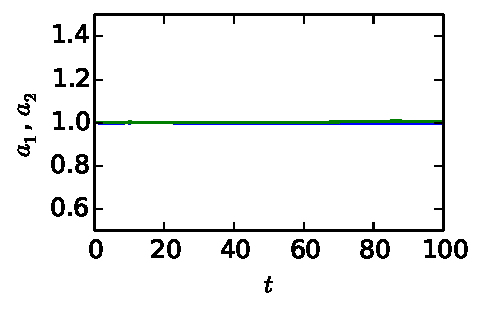
\includegraphics[scale=0.85]{{vlasov_gadget/AxialRatio_0.5}.pdf}
					\centering \caption{Évolution des rapports d'axes $a_1$ et $a_2$ pour $\gamma=-0.5$.\label{Fig::VlaGad::SpheTest::AR}}
					\end{center}
				\end{minipage}\hfill
				\begin{minipage}{0.44\linewidth}
					\begin{center}
					\centering 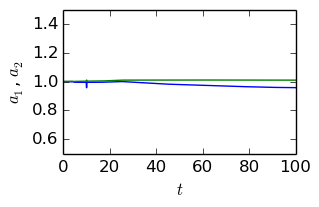
\includegraphics[scale=0.85]{{vlasov_gadget/AxialRatio_0.1}.pdf}
					\centering \caption{Évolution des rapports d'axes $a_1$ et $a_2$ pour
					$\gamma=-0.1$.\label{Fig::VlaGad::SpheTest::AR0.1}}
					\end{center}
				\end{minipage}
				\begin{minipage}{0.44\linewidth}
					\begin{center}
					\centering 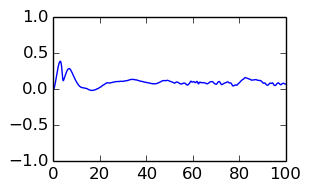
\includegraphics[scale=0.85]{{vlasov_gadget/aniso_0.5}.pdf}
					\centering \caption{Évolution de l'anisotropie pour $\gamma=-0.5$.\label{Fig::VlaGad::SpheTest::Aniso}}
					\end{center}
				\end{minipage}\hfill\hspace{-0.5cm}
				\begin{minipage}{0.44\linewidth}
					\begin{center}
					\centering 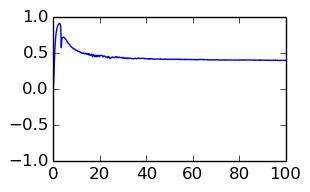
\includegraphics[scale=0.85]{{vlasov_gadget/aniso_0.1}.pdf}
					\centering \caption{Évolution de l'anisotropie pour $\gamma=-0.1$.\label{Fig::VlaGad::SpheTest::Aniso0.1}}
					\end{center}
				\end{minipage}
			\end{figure}

		\label{Sec::VlaGad::Res}
		\subsection{Le cas $\gamma = -0.5$}

		Les panneaux du haut et du milieux des figures~\ref{Fig::ValGad::0.5::t0}, \ref{Fig::ValGad::0.5::t13} et~\ref{Fig::ValGad::0.5::t45} montrent l'évolution de la fonction de distribution dans l'espace des
		phases pour $j=0.425$ et intégrée sur $j$. L'accord entre \textsc{Gadget-2} et \textsc{Vlasolve}
		est très bon jusqu'à $t=45$. À $t=45$, des irrégularités commencent à être visibles dans la structure filamentaire des enroulements de la fonction de distribution dans
		l'espace des phases, ce qui est le signe de l'apparition d'instabilités.
		L'accord entre les deux simulations se déteriore.
		Premièrement, la simulation Vlasov présente comme attendu des effets de diffusion significatifs.
		Deuxièmement, les deux simulations ne semblent plus exactement synchronisées. Notamment, les irrégularités mentionnées plus haut ne sont pas exactement positionnées
		au même endroit.

		Cette désynchronisation n'apparait pas dans les simulations présentées
		dans C2PSS. Les principales différences entre les simulations présentées dans ce chapitre et celles de l'article sont le paramètre de lissage de la force $\epsilon$ et le pas de temps
		maximal autorisé. La figure~\ref{Fig::ValGad::0.5::SoftAll} montre que $\epsilon$ n'a pas d'influence importante sur la dynamique.
		La seule explication du désaccord observé
		est donc le pas de temps, dix fois supérieur ici par rapport aux simulations montrées dans C2PSS.

		Les panneaux du bas des figures~\ref{Fig::ValGad::0.5::t0}, \ref{Fig::ValGad::0.5::t13} et~\ref{Fig::ValGad::0.5::t45} nous
		informent sur l'évolution du profil de densité projetée. Excepté au centre et sur le bord du système, où le nombre de particules devient trop
		faible, l'accord entre \textsc{Vlasolve} et \textsc{Gadget-2} est excellent, même dans les régions de faible densité.
		% la variation relative entre les deux simulations est au pire de l'ordre de $25\%$.

			
		% Un paramètre important de la simulation va être le paramètre de lissage de la force $\epsilon$. Ce paramètre va influencer sur
		% la dynamique en donnant ou retirant de l'importance au collision. Nous avons donc effectué des simulations d'une sphère de
		% Hénon lissée, de viriel $\gamma=-0,5$, avec différents $\epsilon$. La figure~\ref{Fig::ValGad::0.5::SoftAll} montre l'espace
		% des phases pour chaque valeur de $\epsilon$ testées.
		% Nous pouvons voir sur ces figures que l'espace des phases est très similaire, et ne semble pas dépendre de la valeur de
		% $\epsilon$. Les enroulements présentent les mêmes variations et creux quelque soit la valeur de $\epsilon$.

		% Dans la suite, nous prendrons $\epsilon=10^{-3}$. Cette valeur est légèrement différente de celle utilisée pour les simulations
		% de l'article.

		\begin{figure}[htbp]
			\begin{subfigure}{1.00\linewidth}
				\centering \includegraphics[scale=0.75]{{CompVlasGad_t_0_512_0.5}.png}
				% \caption{Comparaison de l'espace des phases entre le code Vlasov (à gauche) et le code Gadget (à droite), à
				% $t=0$ et pour $j=0,425$.\label{Fig::ValGad::0.5::t0}}
			\end{subfigure}\hfill
			\begin{subfigure}{1.0\linewidth}
				\centering \includegraphics[scale=0.75]{{CompVlasGad_t_0_512_0.5_Jall-v2}.png}
				% \caption{$t=0$.\label{Fig::VlaGad::0.5::JAll::t0}}
			\end{subfigure}
			\begin{subfigure}{1.00\linewidth}
				\centering \includegraphics[scale=0.75]{{CompVlasGad_Density_0.5_t_0_error}.pdf}
				%\caption{Comparaison du profil de densité entre le code Vlasov (en bleu) et le code gadget (en vert), pour
				% $t=0$.\label{Fig::ValGad::0.5::Density::t0}}
			\end{subfigure}
			\caption{Comparaison de \textsc{Gadget-2} à \textsc{Vlasolve} pour $\gamma=-0.5$: conditions initiales. En haut: densité dans l'espace des phases pour une tranche de moment angulaire
				dans l'intervalle $j\in[0.4; 0.45]$ (à gauche \textsc{Vlasolve} et à droite \textsc{Gadget-2}); au milieu: densité intégrée sur $j$; en bas: profils de densité projetée $\rho(r)$. La courbe
			bleue correspond au code Vlasov et la courbe verte à la simulation $N$-corps.\label{Fig::ValGad::0.5::t0}}
				% Comparaison du profil de densité entre le code Vlasov (en bleu) et le code gadget (en vert), pour
				% $t=0$.\label{Fig::ValGad::0.5::Density::t0}Comparaison de l'espace des phases entre le code Vlasov (à gauche) et le code Gadget (à droite), à
				% $t=0$ et pour $j=0,425$.\label{Fig::ValGad::0.5::t0}Comparaison du profil de densité entre le code Vlasov (en bleu) et le code gadget (en vert), pour
			% $t=0$.\label{Fig::ValGad::0.5::Density::t0}}
		\end{figure}
		\begin{figure}[htbp]
			\begin{subfigure}{1.00\linewidth}
				\centering \includegraphics[scale=0.75]{{CompVlasGad_t_13_512_0.5}.png}
				% \caption{Comparaison de l'espace des phases entre le code Vlasov (à gauche) et le code Gadget (à droite), à $t=13$ et
				% pour $j=0,425$.\label{Fig::ValGad::0.5::t13}}
			\end{subfigure}\hfill
			\begin{subfigure}{1.0\linewidth}
				\centering \includegraphics[scale=0.75]{{CompVlasGad_t_13_512_0.5_Jall-v2}.png}
				% \caption{$t=13$.\label{Fig::VlaGad::0.5::JAll::t13}}
			\end{subfigure}
			\begin{subfigure}{1.00\linewidth}
				\centering \includegraphics[scale=0.75]{{CompVlasGad_Density_0.5_t_13_error}.pdf}
				% \caption{Comparaison du profil de densité entre le code Vlasov (en bleu) et le code gadget (en vert), pour
				% $t=13$.\label{Fig::ValGad::0.5::Density::t13}}
			\end{subfigure}
			\caption{Comparaison de \textsc{Gadget-2} à \textsc{Vlasolve} pour $\gamma=-0.5$: $t=13$. Suite de la figure~\ref{Fig::ValGad::0.5::t0}.\label{Fig::ValGad::0.5::t13}}
		\end{figure}
		\begin{figure}[htbp]
			\begin{subfigure}{1.00\linewidth}
				\centering \includegraphics[scale=0.75]{{CompVlasGad_t_45_512_0.5}.png}
				% \caption{Comparaison de l'espace des phases entre le code Vlasov (à gauche) et le code Gadget (à droite), à $t=45$ et
				% pour $j=0,425$.\label{Fig::ValGad::0.5::t45}}
			\end{subfigure}\hfill
			\begin{subfigure}{1.0\linewidth}
				\centering \includegraphics[scale=0.75]{{CompVlasGad_t_45_512_0.5_Jall-v2}.png}
				% \caption{$t=45$.\label{Fig::VlaGad::0.5::JAll::t45}}
			\end{subfigure}
			\begin{subfigure}{1.00\linewidth}
				\centering \includegraphics[scale=0.75]{{CompVlasGad_Density_0.5_t_45_error}.pdf}
				% \caption{Comparaison du profil de densité entre le code Vlasov (en bleu) et le code gadget (en vert), pour
				% $t=45$.\label{Fig::ValGad::0.5::Density::t45}}
			\end{subfigure}
			\caption{Comparaison de \textsc{Gadget-2} à \textsc{Vlasolve} pour $\gamma=-0.5$: $t=45$. Suite de la figure~\ref{Fig::ValGad::0.5::t13}.
			\label{Fig::ValGad::0.5::t45}}
		\end{figure}

		\begin{figure}[htbp]
			\begin{subfigure}{0.5\linewidth}
				\centering 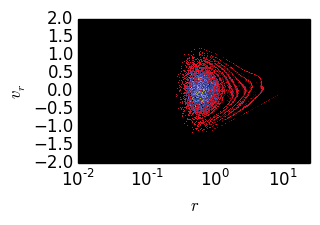
\includegraphics{{vlasov_gadget/Vlasov_0.5_Soft/CompVlasGad_512_0.5_0.0001}.png}
				\centering \caption{$\epsilon=10^{-4}$\label{Fig::ValGad::0.5::Soft1}}
			\end{subfigure}\hfill
			\begin{subfigure}{0.5\linewidth}
				\centering 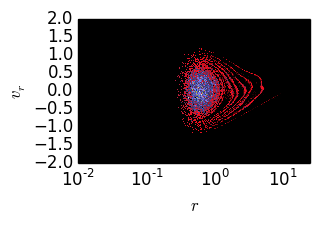
\includegraphics{{vlasov_gadget/Vlasov_0.5_Soft/CompVlasGad_512_0.5_0.001}.png}
				\centering \caption{$\epsilon=10^{-3}$\label{Fig::ValGad::0.5::Soft2}}
			\end{subfigure}
			\begin{subfigure}{0.5\linewidth}
				\centering 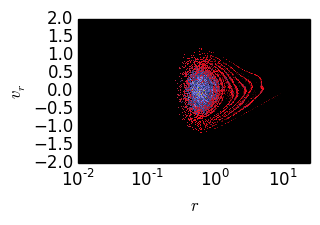
\includegraphics{{vlasov_gadget/Vlasov_0.5_Soft/CompVlasGad_512_0.5_0.01}.png}
				\centering \caption{$\epsilon=10^{-2}$\label{Fig::ValGad::0.5::Soft3}}
			\end{subfigure}\hfill
			\begin{subfigure}{0.5\linewidth}
				\centering 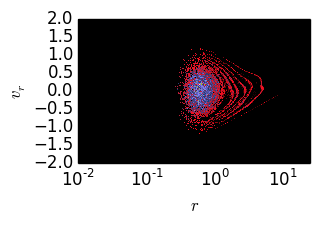
\includegraphics{{vlasov_gadget/Vlasov_0.5_Soft/CompVlasGad_512_0.5_0.1}.png}
				\centering \caption{$\epsilon=10^{-1}$\label{Fig::ValGad::0.5::Soft4}}
			\end{subfigure}
			\caption{Représentation de l'espace des phases à $j=0.425$ et $t=45$ pour $\gamma=-0.5$ et différents
				$\epsilon$.\label{Fig::ValGad::0.5::SoftAll}}
		\end{figure}

		% \begin{figure}[htbp]
			% \begin{subfigure}{1.0\linewidth}
				% \centering \includegraphics[scale=0.75]{{CompVlasGad_t_0_512_0.5_Jall-v2}.png}
				% \caption{$t=0$.\label{Fig::VlaGad::0.5::JAll::t0}}
			% \end{subfigure}
			% \begin{subfigure}{1.0\linewidth}
				% \centering \includegraphics[scale=0.75]{{CompVlasGad_t_13_512_0.5_Jall-v2}.png}
				% \caption{$t=13$.\label{Fig::VlaGad::0.5::JAll::t13}}
			% \end{subfigure}
			% \begin{subfigure}{1.0\linewidth}
				% \centering \includegraphics[scale=0.75]{{CompVlasGad_t_45_512_0.5_Jall-v2}.png}
				% \caption{$t=45$.\label{Fig::VlaGad::0.5::JAll::t45}}
			% \end{subfigure}
			% \caption{Espace des phases intégré sur $j$ pour $\gamma=-0,5$. La simulation Vlasov se trouve à gauche, à droite la simulation gadget.}
		% \end{figure}

		\subsection{Le cas $\gamma = -0.1$}

		Les résultats correspondant à $\gamma=-0.1$ sont similaires aux précédents mais un peu plus complexes. En effet, si nous regardons le profil de densité à
		différents temps (voir les panneaux du bas des figures~\ref{Fig::ValGad::0.1::t0}, \ref{Fig::ValGad::0.1::t5}
		et~\ref{Fig::ValGad::0.1::t25}), l'accord entre \textsc{Gadget-2} et \textsc{Vlasolve} est excellent (toujours à l'exception du centre et du bord du système). Lorsque
		l'on s'intéresse à l'espace des phases, les temps $t\leq10$ (les panneaux du haut et du milieu des figures~\ref{Fig::ValGad::0.1::t0} et~\ref{Fig::ValGad::0.1::t5})
		montrent là encore un excellent accord. Aux temps plus grands, par exemple à $t=25$, comme illustré par la figure~\ref{Fig::ValGad::0.1::t25}, 
		les espaces des phases ne sont plus en aussi bon accord, mais cela n'est pas un problème de synchronisation comme c'était le cas pour $\gamma=-0.5$.
		Ici, on note que la simulation Vlasov, outre une légère diffusion, est sujette à un effet d'aliasing numérique conséquent, mais qui ne semble pas avoir d'effet sur la
		dynamique.
		La simulation \textsc{Gadget-2}, quant à elle, développe une instabilité,
		visible sur les enroulements extérieurs, qui n'est pas présente dans la simulation Vlasov.
		Cette instabilité est étudiée en détail dans C2PSS et nous montrons qu'elle est entièrement due aux effets collectifs du bruit blanc des particules. En effet,
		elle ne dépend ni de $\epsilon$, ni du pas de temps, ni des paramètres contrôlant les erreurs sur la force.
		Il semble de plus qu'elle apparaisse plus tardivement quand on augmente le nombre de particules jusqu'à $N=10^7$. En revanche, une simulation comportant 100 millions
		de particules
		semble aussi instable qu'une simulation n'en comportant que 10 millions. Ceci suggère que l'instabilité observée est bien physique mais se développe trop tôt quand
		le nombre de particules est trop petit. Cette instabilité n'est pas présente dans la simulation \textsc{Vlasolve}, mais cela pourrait être dû aux effets de diffusion
		qui pourraient empêcher certains modes instable de se développer.

		% Les détails à propos du développement de l'instabilité des simulations \textsc{Gadget-2} pourront être trouvés en appendice dans
		% C2PSS. Cette instabilité est due à la nature particulaire de la simulation. L'instabilité
		% apparaissant dans la simulation Vlasov vient d'un mauvais échantillonnage du moment angulaire.

		\begin{figure}[htbp]
			\begin{subfigure}{1.00\linewidth}
				\centering \includegraphics[scale=0.75]{{CompVlasGad_t_0_512_0.1}.png}
				% \caption{Comparaison de l'espace des phases entre le code Vlasov (à gauche) et le code Gadget (à droite), à $t=0$ et pour $j=0,425$.\label{Fig::ValGad::0.1::t0}}
			\end{subfigure}\hfill
			\begin{subfigure}{1.0\linewidth}
				\centering \includegraphics[scale=0.75]{{CompVlasGad_t_0_512_0.1_Jall-v2}.png}
				% \caption{$t=0$.\label{Fig::VlaGad::0.1::JAll::t0}}
			\end{subfigure}
			\begin{subfigure}{1.00\linewidth}
				\centering \includegraphics[scale=0.75]{{CompVlasGad_Density_0.1_t_0_error}.pdf}
				% \caption{Comparaison du profil de densité entre le code Vlasov (en bleu) et le code gadget (en vert), pour $t=0$.\label{Fig::ValGad::0.1::Density::t0}}
			\end{subfigure}
			\caption{Comparaison de \textsc{Gadget-2} à \textsc{Vlasolve} pour $\gamma=-0.1$: conditions initiales. En haut: densité dans l'espace des phases pour une tranche de moment angulaire
				dans l'intervalle $j\in[0.4; 0.45]$ (à gauche \textsc{Vlasolve} et à droite \textsc{Gadget-2}); au milieu: densité intégrée sur $j$; en bas: profils de densité projetée $\rho(r)$. La courbe
				bleue correspond au code Vlasov et la courbe verte à la simulation $N$-corps.
			\label{Fig::ValGad::0.1::t0}}
		\end{figure}
		\begin{figure}[htbp]
			\begin{subfigure}{1.00\linewidth}
				\centering \includegraphics[scale=0.75]{{CompVlasGad_t_5_512_0.1}.png}
				% \caption{Comparaison de l'espace des phases entre le code Vlasov (à gauche) et le code Gadget (à droite), à $t=5$ et pour $j=0,425$.\label{Fig::ValGad::0.1::t5}}
			\end{subfigure}\hfill
			\begin{subfigure}{1.0\linewidth}
				\centering \includegraphics[scale=0.75]{{CompVlasGad_t_5_512_0.1_Jall-v2}.png}
				% \caption{$t=5$.\label{Fig::VlaGad::0.1::JAll::t5}}
			\end{subfigure}
			\begin{subfigure}{1.00\linewidth}
				\centering \includegraphics[scale=0.75]{{CompVlasGad_Density_0.1_t_5_error}.pdf}
				% \caption{Comparaison du profil de densité entre le code Vlasov (en bleu) et le code gadget (en vert), pour $t=5$.\label{Fig::ValGad::0.1::Density::t5}}
			\end{subfigure}
			\caption{Comparaison de \textsc{Gadget-2} à \textsc{Vlasolve} pour $\gamma=-0.1$: $t=5$. Suite de la figure~\ref{Fig::ValGad::0.1::t0}.
				\label{Fig::ValGad::0.1::t5}}
		\end{figure}
		\begin{figure}[htbp]
			\begin{subfigure}{1.00\linewidth}
				\centering \includegraphics[scale=0.75]{{CompVlasGad_t_25_512_0.1}.png}
				% \caption{Comparaison de l'espace des phases entre le code Vlasov (à gauche) et le code Gadget (à droite), à $t=25$ et pour $j=0,425$.\label{Fig::ValGad::0.1::t25}}
			\end{subfigure}\hfill
			\begin{subfigure}{1.0\linewidth}
				\centering \includegraphics[scale=0.75]{{CompVlasGad_t_25_512_0.1_Jall-v2}.png}
				% \caption{$t=25$.\label{Fig::VlaGad::0.1::JAll::t25}}
			\end{subfigure}
			\begin{subfigure}{1.00\linewidth}
				\centering \includegraphics[scale=0.75]{{CompVlasGad_Density_0.1_t_25_error}.pdf}
				% \caption{Comparaison du profil de densité entre le code Vlasov (en bleu) et le code gadget (en vert), pour $t=25$.\label{Fig::ValGad::0.1::Density::t25}}
			\end{subfigure}
			\caption{Comparaison de \textsc{Gadget-2} à \textsc{Vlasolve} pour $\gamma=-0.1$: $t=25$. Suite de la figure~\ref{Fig::ValGad::0.1::t5}.
			\label{Fig::ValGad::0.1::t25}}
		\end{figure}
		% \begin{figure}[htbp]
			% \begin{minipage}{1.00\linewidth}
				% \centering \includegraphics[width=\linewidth]{{CompVlasGad_t_35_512_0.1}.png}
				% \caption{Comparaison de l'espace des phases entre le code vlasov (à gauche) et le code Gadget (à droite), à $t=35$ et
				% pour $j=0,425$.\label{Fig::ValGad::0.1::t35}}
			% \end{minipage}\hfill
			% \begin{minipage}{1.00\linewidth}
				% \centering \includegraphics{{CompVlasGad_Density_0.1_t_35_error}.pdf}
				% \caption{Comparaison du profil de densité entre le code vlasov (en bleu) et le code gadget (en vert), pour $t=35$.\label{Fig::ValGad::0.1::Density::t35}}
			% \end{minipage}
		% \end{figure}

		% \begin{figure}[htbp]
			% \begin{subfigure}{1.0\linewidth}
				% \centering \includegraphics[scale=0.75]{{CompVlasGad_t_0_512_0.1_Jall-v2}.png}
				% \caption{$t=0$.\label{Fig::VlaGad::0.1::JAll::t0}}
			% \end{subfigure}
			% \begin{subfigure}{1.0\linewidth}
				% \centering \includegraphics[scale=0.75]{{CompVlasGad_t_5_512_0.1_Jall-v2}.png}
				% \caption{$t=5$.\label{Fig::VlaGad::0.1::JAll::t5}}
			% \end{subfigure}
			% \begin{subfigure}{1.0\linewidth}
				% \centering \includegraphics[scale=0.75]{{CompVlasGad_t_25_512_0.1_Jall-v2}.png}
				% \caption{$t=25$.\label{Fig::VlaGad::0.1::JAll::t25}}
			% \end{subfigure}
			% \caption{Espace des phases intégré sur $j$ pour $\gamma=-0,1$. La simulation Vlasov se trouve à gauche, à droite la simulation gadget.}
		% \end{figure}



	\section{Discussion}
		\label{Sec::VlaGad::Art}

		% Pour comparer nos simulations, nous regarderons la correspondance entre l'espace des phases $(r, v_r)$ pour $j=0,425$, l'espace
		% des phases intégré sur $j$ et le profil de densité de l'objet. Nous effectuerons ces comparaison à différents temps afin
		% de montrer que nous obtenons bien le même comportement au cours de l'évolution du système. La simulation \textsc{gadget-2} utilisée ici comporte $10^6$
		% particules. L'article associé étudie aussi l'évolution de simulations composées de $10^5$ et $10^7$ particules.

		Dans ce chapitre, nous venons de comparer \textsc{Gadget-2} à un code Vlasov et les résultats de nos analyses, tant pour l'inspection visuelle dans l'espace des phases
		que pour le profil de densité $\rho(r)$, montrent un bon accord général entre les deux méthodes numériques à condition d'utiliser les bons paramètres pour réaliser les
		simulations. Nous notons cependant l'apparition d'une instabilité numérique dans les simulations \textsc{Gadget-2} dans le cas $\gamma=-0.1$. Cette instabilité
		pourrait être
		physique bien que dans C2PSS, nous ayons montré une dépendance manifeste par rapport au nombre de particules utilisées dans les simulations $N$-corps.
		
		Ici, j'ai utilisé des simulations avec $N=10^6$ particules et je n'ai testé que les variations (très faibles) induites par le choix du lissage de la force. Dans
		C2PSS, des tests supplémentaire sont réalisés, notamment en variant le nombre de particules entre $N=10^4$ et $N=10^8$, le pas de temps et les
		paramètres de tolérance sur l'erreur de la force. Clairement, la quantité la plus déterminante est le nombre de particules. En particulier, il semble
		nécessaire d'avoir au moins de l'ordre de 100 millions de particules pour réaliser correctement une simulation de la sphère de Hénon avec $\gamma=-0.1$!

		Dans C2PSS, des analyses quantitatives supplémentaires sont réalisées pour compléter l'inspection visuelle de la fonction de distribution dans l'espace des phases.
		Pour réaliser ces mesures additionnelles, de nouveaux estimateurs statistiques sont introduits: des corrélateurs et des estimateurs de l'entropie, tous deux basés sur
		une écriture de la vraisemblance que les simulations $N$-corps représentent des réalisations localement poissoniennes des simulations Vlasov.
		L'analyse statistique confirme les impressions visuelles et apporte quelques informations supplémentaires. Notamment, on remarque que pendant la phase de relaxation,
		l'accord entre les simulations $N$-corps et les simulations Vlasov se dégrade temporairement. Cet évènement est de plus faible amplitude et apparaît plus
		tardivement quand le nombre de particules augmente.

		Ce qu'il faut conclure de ce chapitre, c'est que les simulations $N$-corps sont capables dans les cas relativement chauds considérés ici de suivre avec précision la
		structure fine
		de l'espace des phases, mais il est nécessaire d'utiliser un grand nombre de particules et cela d'autant plus que le système est froid.


	% Au cours des deux dernières sous-sections, nous venons de comparer deux simulations, l'une effectuée avec un code Vlasov, l'autre avec
	% \textsc{Gadget-2}. L'accord entre ces deux simulations, même à faible viriel, est excellent. Pour le cas $\gamma=-0.1$, il est difficile de
	% réellement conclure, puisque des instabilités numériques se produisent relativement tôt dans la simulation, même si la correspondance observée
	% avant semble optimiste.





		% Le premier temps que nous regardons est $t=0$. La figure~\ref{Fig::ValGad::0.5::t0} Du côté du profil de densité
		% (figure~\ref{Fig::ValGad::0.5::Density::t0}), l'accord est très bon, excepté au centre du système où le manque de particules empêche
		% le calcul précis de la densité.
		% Le deuxième temps que nous avons choisi de montrer se situe peu après la fin de l'effondrement de la sphère de Hénon. Le nombre
		% d'enroulement présent sur les graphiques de la figure~\ref{Fig::ValGad::0.5::t13} sont les mêmes. Par contre, l'enroulement central
		% donne de la simulation gadget semble un peu en avance sur la simulation vlasov. Ce qui semble confirmé par le \og{}bras\fg s'étendant
		% jusqu'à $r=3$ pour la simulation vlasov et jusqu'à $r=4$ pour la simulation gadget.
		% Les profils de densité présenté sur la figure~\ref{Fig::ValGad::0.5::Density::t13} montre par contre un très bon accord, excepté au
		% bord du système, où le nombre de particules recommence alors à faiblir. L'extension du système en $r$ est aussi visible.
		% Cette extension du profil peut-être expliqué par l'éjection d'une fraction des particules hors du système suite aux collisions se
		% produisant dans le système.
		% Pour terminer la comparaison à ce viriel, nous regardons ce qu'il se passe à $t=45$. À ce moment, le système a eu le temps de se
		% stabiliser. Nous remarquons, en regardant la figure~\ref{Fig::ValGad::0.5::t45}, que la simulation gadget présente des
		% \og{}vaguelettes\fg sur les enroulements extérieurs qui semble en avance sur la simulation vlasov.


		% Le premier temps que nous regardons est $t=0$. La figure~\ref{Fig::ValGad::0.1::t0} montre l'espace des phases pour les conditions
		% initiales. La première chose à noter concerne la différence apparente concernant le maximum de la fonction de distributions. Cette
		% différence est dû au faible nombre de particules présentes dans la couche de $j$ choisi. Excepté ce point, nous retrouvons bien la
		% croissance progressive du nombre de particule ainsi qu'un étalement progressif des vitesses radiales quand $r$ augmente.
		% Du côté du profil de densité (figure~\ref{Fig::ValGad::0.1::Density::t0}), l'accord est très bon, excepté au centre du système où le manque de particules empêche le calcul précis
		% de la densité.

		% Le deuxième temps que nous avons choisi de montrer se situe peu après la fin de l'effondrement de la sphère de Hénon. Le nombre
		% d'enroulement présent sur les graphiques de la figure~\ref{Fig::ValGad::0.1::t13} sont les mêmes. Par contre, l'enroulement central
		% donne de la simulation gadget semble un peu en avance sur la simulation vlasov. Ce qui semble confirmé par le \og{}bras\fg s'étendant
		% jusqu'à $r=3$ pour la simulation vlasov et jusqu'à $r=4$ pour la simulation gadget.
		% Les profils de densité présenté sur la figure~\ref{Fig::ValGad::0.1::Density::t13} montre par contre un très bon accord, excepté au
		% bord du système, où le nombre de particules recommence alors à faiblir. L'extension du système en $r$ est aussi visible.
		% Cette extension du profil peut-être expliqué par l'éjection d'une fraction des particules hors du système suite aux collisions se
		% produisant dans le système.

		% Pour terminer la comparaison à ce viriel, nous regardons ce qu'il se passe à $t=45$. À ce moment, le système a eu le temps de se
		% stabiliser. Nous remarquons, en regardant la figure~\ref{Fig::ValGad::0.1::t45}, que la simulation gadget présente des
		% \og{}vaguelettes\fg sur les enroulements extérieurs qui semble en avance sur la simulation vlasov.
